\documentclass[12pt]{article}
\usepackage{graphicx}
\usepackage{amsmath,amsfonts,amssymb}

\title{Local Extrema Relationships to Shape Features}
\author{Michael Deakin}
\date{\today}

\begin{document}
\maketitle
In this project, I looked at using the methods covered in class to find new ways of understanding a local optimization problem.
The problem relies on several definitions.
Given a curve $C$ and a point on the curve $C(s)$, the local minima are defined as all points $C(t)$ such that $\frac{\partial|C(t)-C(s)|}{\partial t}=0$ and $\frac{\partial^2|C(t)-C(s)|}{\partial t^2}>0$.
A continuous movement of the local minimum is defined as small changes in $t$ for small changes in $s$ such that the previous constraints are preserved.
In other words, if $\exists \epsilon_s>0$ s.t. $\forall \Delta s<\epsilon_s, \exists \Delta t\propto \Delta s$ where $\frac{\partial|C(t+\Delta t)-C(s + \Delta s)|}{\partial t}=0$ and $\frac{\partial^2|C(t+\Delta t)-C(s+\Delta s)|}{\partial t^2}>0$, $\Delta t$ is a continuous movement of the minimum for a movement $\Delta s$ of the reference point.
Two types of discontinuous movements of a local minimum are defined.
The first occurs whenever the reference point crosses the evolute of the curve.
This corresponds to the annihilation and creation events of a local minimum and maximum pair.
The creation event is uninteresting for our problem, and will be ignored.
The second type of discontinuous movement occurs when there exists two distinct values $u$ and $v$ such that $C(u)=C(v)$.
In this case, after some movement of the minima at $C(u)$ and $C(v)$, if $|C(u+\Delta u)-C(s+\Delta s)|<|C(v+\Delta v)-C(s+\Delta s)|$, the minimum at $C(v)$ has a discontinuous movement to $C(u+\Delta u)$.
The problem can then be defined as follows:
Is there a curve $C$, starting point $s_0$, starting minimum $t_0\neq s_0$, and continuous movement function $ds$ where $s=s_0+\int ds$, $\int ds=L(C)$, $t=t_0+\int m(s, t) ds$, and $t_f=t_0$?\\
\begin{figure}
\centering
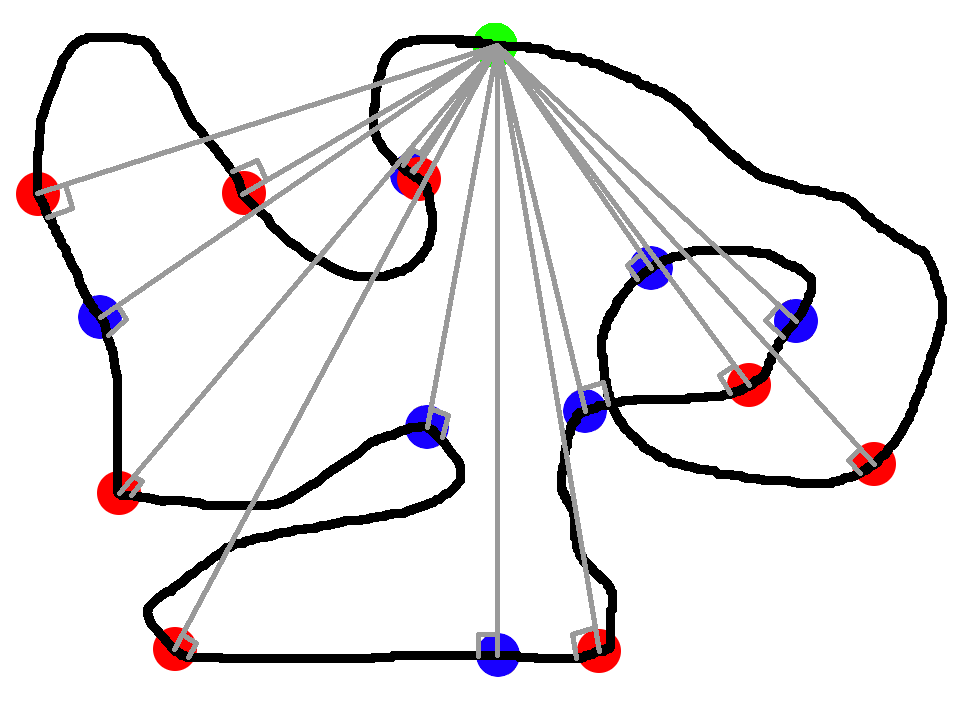
\includegraphics[width=200px]{project_problem.png}
\caption{Example Curve with Minima and Maxima wrt. a Reference Point}
\end{figure}
This problem does not yield if attacked directly, so this project attempts simplifies it to look at extremes.
I attempted to look at the extremes from a multidimensional surfaces point of view.
To do this, I looked at the shape of $D=C\times C$, and tried to come up with correlations to different features on the surface.
This turns out to be a rather interesting family of shapes, because features which are generally non-generic are generic here.\\
The first thing I did with this shape was compute its principal directions.
The principal directions turn out to be directly related to the tangent directions of the curve.
For a point $D(s, t)$, these are $(\frac{\partial D(s, t)}{ds}, (0, 0))$ and $((0, 0), \frac{\partial D(s, t)}{dt})$.\\
This can be seen quite easily by considering the tangent directions defined by $s$ and $t$ at a point.
Changing $s$ only changes the tangent corresponding to $s$, and similarly for $t$.
Thus, there is no ``twist'' as one moves in the $s$ direction on the surface or in the $t$ direction, satisfying the definition of a principal direction.\\
This means that approximating the movement of a local minimum with respect to the reference point translates exactly to the relationship of a minimum and the principal directions at it's point.\\
A simple approximation of the movement of a local extreme can be created by considering the osculating circle at the point of the extreme.
\begin{figure}
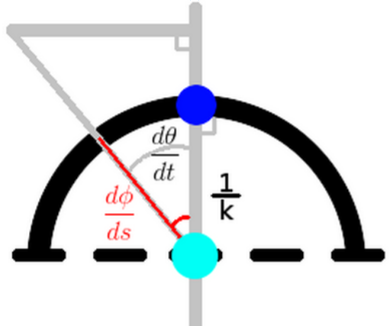
\includegraphics[width=200px]{project_osculating_approx.png}
\caption{Model for Approximating an Extremes Movement}
\end{figure}
Assuming the extreme lies on a region of constant curvature, it must move at the same angular rate as the reference point with respect to the osculating circle's center.
This is required to maintain the orthogonality constraint.
We can then compute the angular ``velocity'' of the reference point as $\omega=\frac{dC(s)}{dt}\times \vec{r}/|\vec{r}|^2$, where $\vec{r}$ is the displacement from the center of the osculating circle to the reference point.
The angular velocity is the same for the minimum, so we just compute the linear velocity as $\frac{\omega}{\kappa(t)} \frac{dC(t)}{dt}/|\frac{dC(t)}{dt}|$.
This model is a rather nasty differential equation, but can be made nicer by not considering the original parameters of the shape.
By simply looking at the movement in the coordinate space defined by the tangent direction of the minimum point, we can say approximately how far in the tangent space the extreme moves.
Let $x=\frac{dC(s)}{dt}\times \vec{r}/|\vec{r}|, \theta =\arctan\left (\frac{x}{|\vec{r}|} \right)$.
Then $\lambda=\frac{d\theta}{dx}=\frac{|\vec{r}|}{|\vec{r}|^2+x^2|}$.
For the minimum, note $\phi=\arctan\left(\frac{u}{\kappa}\right), \lambda=\frac{d\phi}{du}=\frac{\kappa}{\kappa^2+u^2}$.
Then $u=\pm\sqrt{\kappa |\vec{r}|+\frac{\kappa^2}{|\vec{r}|}x^2-\kappa^2}$.
Since the minimum is on a region of constant curvature, the radial direction does not have any component, and the result is in the second principal direction.
Thus we have completely defined an approximation of the movement of an extreme in terms of the principal directions.
This is a semi-linear relationship between the direction a minimum moves with respect to the reference point, which implies its a model of first order accuracy.\\
After constructing the relationship for principal directions, it seemed like a good idea to look at the asymptotic directions.
By Euler's Formula, $k=\kappa_1\cos^2(\theta)+\kappa_2\sin^2(\theta)$.
Since we want $k=0$, we find that $\theta=\pm\arctan\left(\sqrt{-\frac{\kappa_1}{\kappa_2}}\right)$.
Then the asymptotic directions are \\$\left(\sqrt{-\frac{\kappa_1}{\kappa_1+\kappa_2}}\frac{dC(s)}{dx}, \sqrt{-\frac{\kappa_1}{\kappa_1+\kappa_2}}\frac{dC(s)}{dy}, \pm\sqrt{-\frac{\kappa_2}{\kappa_1+\kappa_2}}\frac{dC(t)}{dx}, \pm\sqrt{-\frac{\kappa_2}{\kappa_1+\kappa_2}}\frac{dC(t)}{dy}\right)$.
Comparing this to the relationship between the movement of the minimum and the principal directions, we see that the asymptotic directions don't have anything to do with the distance from the osculating circle (not surprising), and are unrelated beyond a rather lengthy change in coordinates.\\
After this, I considered the movement of the local extreme at various objects of interest.
On parabolic curves with the same color as the minimum's principal direction, the movement of the local minimum exactly matches the parallel movement of the reference point.
On the other parabolic curves, there is not any nice relationship, the relationship derived for principal directions must be used.
For features which are generically points, a local minimum corresponding to one of those points happens to be non-generic, and thus they were not considered further.
The umbilic happens to be a special exception to this rule.
An unavoidable consequence of this method of constructing surfaces is that there is a ``curve'' of umbilics on the surface.
In this case, this curve coincides with the global minimum.
In the parameter space, this has a constant direction of (1, 1).
This is the only generic curve of umbilics, however, and we are not considering the global minimum, so this interesting fact is of little use.
Another weird point in this family of surfaces is the parabolic umbilic.
This one is also not generic except in the global minimum case, where it occurs in transitions between convex and concave regions of the curve.\\
\end{document}
